\chapter{Model Design}	\label{chap:model}
	In earlier chapters we have identified the processes of the Status, Sensors, Safety and Hardware Controller.
	We have kept these processes separated according to the identified processes.
	The list of processes is as follows:
	\begin{description}
		\item[SafetyController] the controller responsible for security:
			\begin{description}
				\item[SafetyPreSigns] handles the safety aspect of the pre-signs.
				\item[SafetyStopSigns] idem for the stop signs.
				\item[SafetyBarriers] idem for the barriers.
				\item[SafetyDeck] idem for the deck.
					\begin{description}
						\item[SafetyDeck\_Pins] component of the deck safety controller that handles the pins.
						\item[SafetyDeck\_Brakes] idem for the brakes.
						\item[SafetyDeck\_Motor] idem for the motor.
					\end{description}
			\end{description}
		\item[HardwareController] the controller responsible for modelling the hardware layer.
		\item[StatusController] the controller responsible for storing the sensor status of bridge components.
		\item[Sensors] models the sensor behaviour. 
	\end{description}



	The resulting LTS model has $170$ levels, $247,940$ states and $358,268$ transitions.
	The number of states exploded when we added code for processing the sensor handling.
	In particular the code given in~\cref{list:sensorpolling} causes a large number of states,
	because of the many types of values the variables can assume: $3^{12}\cdot4 > 2\cdot 10^6$.
	Additionally, a graphical representation of the state space is given in~\cref{fig:statespace}

	\lstinputlisting[style=MCRL2, caption={The polling of sensor state in the StatusController}, label={list:sensorpolling}]{source/sensorpolling.mcrl2}

	\begin{figure}[h]
		\centering
		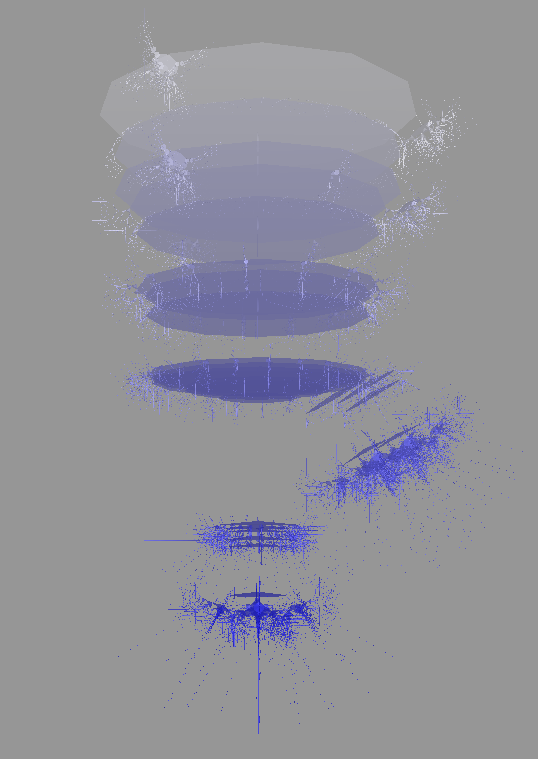
\includegraphics[height=0.4\textheight]{images/state_model.png}
		\caption{3D State space model of the entire system}
		\label{fig:statespace}
	\end{figure}

	\section{Safety Controller}
		The safety controller has several sub-processes handling the behaviour of each possible user input.		
		Because we assumed that the user has only inputs for pre-signs,
		stop-signs, barriers and the bridge deck there are only 4 of these sub-processes.
 
		Each sub-process first checks if the relevant component does not have the \texttt{error} sensor state.
		Then, depending on the user input, the required state is checked,
		e.g. for turning the stop signs on the pre-signs have to be on.
		But for turning the stop signs off the barriers have to be off instead.
		Then the Hardware Controller is requested to execute the user request,
 if the state is as expected.
 	 A Produce OK (\texttt{ProdOK}) is executed if everything went as expected,
 	 Produce Error (\texttt{ProdError}) if a requirement was not met.

 	 The deck safety controller was split into several sub-processes,
 	 because opening the bridge deck is a complex interplay of three bridge components:
 	 the locking pins, the brakes and the motor.
 	 To save space we introduced a \texttt{Direction} type as additional argument,
 	 which allows us to reuse the sub-process in both up and downward operation of the bridge deck.
 	 While the number of branches can be large at times (see \texttt{SafetyDeck\_Motor}),
 	 the behaviour is simple and very similar to a finite state machine. 

	\section{Hardware Controller}
		The goal of the hardware controller is modelling the hardware behaviour.
		All this does in our system is setting the sensor status of the requested component to the correct type.
		This process could be extended to perform hardware routines.

	\section{Status Controller}
		The status controller offers both functionality to poll sensor data and aggregate the results,
		and to read the aggregated data that is saved in its state.
		We use a polling method for reading the sensors,
		because analysing this is easier than an asynchronous process that can update the state at any time.

		The polling of all sensors is performed in one block of code after a \texttt{startUpdateStatus} request.
		Even though this is not very efficient in the number of the states,
		the code remains well readable this way.
		The status of the signs are stored inside \texttt{Bag} objects,
		which we can later use to calculate the number of \texttt{on}, \texttt{off} and \texttt{error} states of the signs.
		After polling the sensors, this data is saved in the state of the status controller for later reading.

		The reading can be done with a \texttt{checkStatusX} request,
		where $X$ is a component.
		This is straightforward reading from the current state of the status controller,
		except for the signs.
		The signs have as additional requirement that if just one sign has an error sensor state,
		that the bridge can still remain operational.
		To this end we created the Bags at the sensor polling phase,
		because now it is easy to count the number of occurrences of states in and conclude the appropriate aggregated sign state.
		
		The initial values of the status of the components are given in \cref{tbl:statusinit}.
		
		\begin{table}[!htbp]
			\begin{center}
			\begin{tabular}{l l}
				\hline
				Status				& Value	\\
				\hline
				statusPreSignBag	&	{off:4, on: 0, error:0}		\\
				statusStopSignBag	&	{off:4, on:0, error:0}		\\
				statusBarriers		&	off		\\
				statusBrakes		&	on		\\
				statusPins			&	on		\\
				statusDeck			&	off		\\
				statusMotor			&	status\_stopped	\\
				\hline
			\end{tabular}
			\caption{The initial values of the status of the components}
			\label{tbl:statusinit}
			\end{center}
		\end{table}

	\section{Sensors} \label{sec:sensors}
		The sensors are a simple sub-process that keep track of the current sensor state of the components.
		When the hardware changes it notifies the sensors so that the state may be updated.
		Requests to the sensors can be achieved with \texttt{commSensorX} action. 
		To model possible defects in the system, there is a possibility to return an \texttt{error} state for each communication.
		This way it is possible for a sensor to return an error state independent of the hardware controller.
		The sensor are initialized with the values as listed in \cref{tbl:sensorinit}.
		
		\begin{table}[!htbp]
			\begin{center}
			\begin{tabular}{l l}
				\hline
				Sensor	& Value	\\
				\hline
				sensorPreSigns	&	off	\\
				sensorStopSigns	&	off	\\
				sensorBarriers	&	off	\\
				sensorPins		&	on	\\
				sensorBrakes	&	on	\\
				sensorDeck		&	off	\\
				sensorMotor		&	status\_stopped\\
				\hline
			\end{tabular}
			\caption{The initial value of the sensors}
			\label{tbl:sensorinit}
			\end{center}
		\end{table}
	

	\section{Initialization}
		In \cref{list:initialization} the initialization of the processes in our model is given. Also all actions that are allowed and the corresponding communicating actions are declared here. Finally the parallel processes are initialized with the correct initial values for the sensors and the status of all the components.
		The various controllers are run in parallel and synchronized using the communication actions.
		The initial state of the model is set in both the \texttt{StatusController} as well as the \texttt{Sensors}.
		For the \texttt{StatusControler} it is assumed that:
		\begin{enumerate}
			\item all the signs are off
			\item the barriers are open (off)
			\item the brakes are on
			\item the pins are engaged (on)
			\item the deck is down (off)
			\item the motor is off (status\_stopped)
		\end{enumerate}
		The same holds for the initial state of the \texttt{Sensors}.
		
		\lstinputlisting[style=MCRL2, caption={The initialization of the mCRL2 model.}, label={list:initialization}]{source/initialization.mcrl2}